\documentclass[12pt]{report}
\usepackage[a4paper]{geometry}
\usepackage[myheadings]{fullpage}
\usepackage{fancyhdr}
\usepackage{lastpage}
\usepackage{graphicx, wrapfig, subcaption, setspace, booktabs}
\usepackage[T1]{fontenc}
\usepackage[font=small, labelfont=bf]{caption}
\usepackage{fourier}
\usepackage[protrusion=true, expansion=true]{microtype}
\usepackage[english]{babel}
\usepackage{sectsty}
\usepackage{url, lipsum}


\newcommand{\HRule}[1]{\rule{\linewidth}{#1}}
\onehalfspacing



%-------------------------------------------------------------------------------
% HEADER & FOOTER
%-------------------------------------------------------------------------------
\pagestyle{fancy}
\fancyhf{}
\setlength\headheight{15pt}
\fancyhead[L]{SDD}
\fancyhead[R]{College of Engineering,Trivandrum}
\fancyfoot[R]{Page \thepage\ of \pageref{LastPage}}
%-------------------------------------------------------------------------------
% TITLE PAGE
%-------------------------------------------------------------------------------
\begin{document}

\title{ \normalsize \textsc{Department of Computer Science}
		\\ [2.0cm]
		\HRule{0.5pt} \\
		\LARGE \textbf{\uppercase{Software Design Document}}
		\HRule{2pt} \\ [0.5cm]
		\normalsize \today \vspace*{5\baselineskip}}

\date{}

\author{
		Aarya R Shankar \\ 
		Amrith M \\
		Anand R \\
		Sarathchandran S }

\maketitle

\newpage

%-------------------------------------------------------------------------------
% Section title formatting
\sectionfont{\scshape}
%-------------------------------------------------------------------------------

%-------------------------------------------------------------------------------
% BODY
%-------------------------------------------------------------------------------

\section*{Introduction}
The aim of the project is to create an character recognition system for Malayalam language. Character recognition systems have been developed for many other languages and is used in various applications. Tesseract is an OCR system implemented for English language. We think it is high time that Malayalam has one too.

In this project, we will create a classifier that classifies Malayalam alphabets using Convolutional Neural Networks. Malayalam Language has 51 letters primarily. These 51 letters are not enough for a character recognition system for this language as various symbols and their combinations are used commonly. Thus, we create a system with 133 classes which includes all the symbols that appear in the language. 

%-------------------------------------------------------------------------------
% REFERENCES
%-------------------------------------------------------------------------------
\section*{High Level Entities}
The project requires a large set of images of individual Malayalam characters. Multiple images of each character is collected and a deep learning model is trained with the help of the available dataset. We rely on neural networks for this. With the availability of huge computational capability, deep learning has proven its strength in diverse domains. We design a convolutional neural network model to train on the dataset and then fine tune the hyperparameters of the model based on the validation accuracy. From formatting the images to building the model and saving the weights of the network, the entire process happens in python. 

\section*{Low Level Entities}
\subsection*{Dataset Collection and Preparation}
The dataset of 133 Malayalam characters were collected from SPACE (Society for Promotion of Alternative Computing and Employment). It contained varying quantity of images belonging to each Malayalam character and in varying dimensions. To develop a model, the image data should have uniformity in the number of color channels and in the size of the training image. We converted all the images into grayscale and their size to 32x32 pixels. 
\subsection*{Preparing the model}

An initial convolutional Neural Network model is designed to work with the current dataset. A Convolutional Neural Network (CNN) has the following  layers: convolutional layers, pooling layers, and fully connected layers. CNNs use variation of multilayer perceptrons designed to require minimal preprocessing. They are also known as shift invariant or space invariant artificial neural networks. Convolutional layers apply a convolution operation to the input, passing the result to the next layer. Convolutional networks may include local or global pooling layers, which combine the outputs of neuron clusters at one layer into a single neuron in the next layer. This is done for downsampling a feature map obtained as the output of a convolutional layer. The final fully connected layers connects every neuron in the previous layer to the next layer. So the final downsampled feature map is stretched into a single vector and is given as input to the fully connected layer. The output of the final fully connected layer contains the required number of classes. 

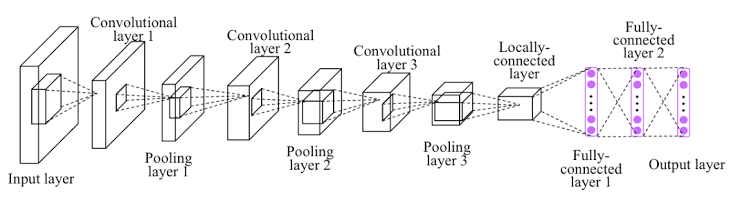
\includegraphics[width=\textwidth]{cnn.png}

\subsection*{Estimating the performance}
The weights of the the above designed model are saved and the model is tested against a validation set. The validation set is usually a separate partition of the dataset which is not used for training. To improve the accuracy, the hyperparameters such as learning rate are tweaked. If the performance does not improve, the architecture will be tweaked as well. Once the model is found to show decent accuracy, the weights can be saved and used for character classification. 

\section*{Benefits}
\begin{itemize}
\item First and foremost, we can use this to develop an OCR for Malayalam language.


\item Our Kerala Government has enlisted Malayalam as the language of all official documents. Hence, a malayalam OCR is necessary for digitalising them efficiently. Our model can speed up its development process by a considerable factor.
\item This project may be modified to read the malayalam scripts and process them using NLP (Natural Language Processing) and use a text-to-speech software as an aid to blind people.
\end{itemize}

\section*{Risks}
\begin{itemize}
\item The biggest problem in developing a model is that if the dataset is not good enough, the model will not be good enough. Hence the dataset to be prepared must have the various characters and their combinations.
\item Training a large set of dataset needs a very efficient GPU, which is not easily available.

\end{itemize}


\section*{Conclusion}


 Considering all the entities, benefits and the risks of this project, we can conclude that our project is a probable one and will also be a beneficial one to the society.


\end{document}